\chapter{Statistics}\label{chapter:stats}

This chapter provides an overview of the statistics used in LingPipe
as well as the statistical utilities provided as classes and methods
by LingPipe.  Without the space to repeat an entire calculus, matrix
and math stats curriculum, we use this appendix more as a reminder for
the definitions we use in the book.

\section{Useful Functions}


\subsection{Logarithms and Exponents}

The exponential function $\exp(x)$ is defined as the unique non-zero
solution to the differential equation
%
\begin{equation}
\frac{d}{dx}f = f.
\end{equation}
%
That is, $\exp(x)$ is the unique function satisfying this equation.
The exponential function may be applied to any real number, but its
value is always positive.  The exponential function has some
convenient properties, such as
%
\begin{equation}
\exp(a + b) = \exp(a) \times \exp(b), \mbox{ and}
\end{equation}
%
\begin{equation}
\exp(a \times b) = \exp(a)^b.
\end{equation}

The natural logarithm, $\log x$ is defined as the inverse of $\exp(x)$,
taking
%
\begin{equation}
\log \exp(x) = x.
\end{equation}
%
For all $y > 0$, we also have $\exp(\log y) = y$.  Logarithms convert
multiplication into addition and exponentiation into multiplication, with
%
\begin{equation}
\log (x \times y) = \log x + \log y, \mbox{ and}
\end{equation}
%
\begin{equation}
\log x^y = y \log x.
\end{equation}



\subsection{The Factorial Function}\label{section:stats-factorial}

The factorial function computes the number of different ordered
permutations there are of a list of a given (non-negative) number of
distinct objects.  The factorial function is written $n!$
and defined for $n \in \nats$ by
%
\begin{equation}
n! = 1 \times 2 \times \cdots \times n = \prod_{m=1}^n m.
\end{equation}
%
The convention is to set $0! = 1$ so that the boundary conditions of
definitions like the one we provided for the binomial coefficient work
out properly.


\subsection{Binomial Coefficients}\label{section:stats-binomial-coefficient}

The binomial coefficient has many uses.  We're mainly interested in
combinatorics, so we think of it as providing the number of ways to
select a subset of a given size from a superset of a given size.  The
binomial coefficient is written ${m choose n}$, prounced ``$m$
choose $n$,'' and defined for $m, n \in \nats$ with $n \geq m$ by
%
\begin{equation}
{n \choose m} = \frac{n!}{m! \ (n-m)!}.
\end{equation}


\subsection{The $\Gamma$ Function}\label{section:stats-gamma-function}

The $\Gamma$ function is the complex generalization of the factorial
function (see \refsec{stats-factorial}).  It is written $\Gamma(x)$, 
and we're only concerned with real $x \in [0,\infty)$, where its value
is defined by 
%
\begin{equation}
\Gamma(x) = \int_0^{\infty} t^{x-1} \ \exp(-t) \ dt.
\end{equation}
%
In general, we have
%
\begin{equation}
\Gamma(x+1) = x \ \Gamma(x).
\end{equation}
%
Because we have $\Gamma(1) = 1$, we also have for all $n \in \nats, n > 0$, 
%
\begin{equation}
\Gamma(n) = (n-1)!.
\end{equation}


\section{Discrete Probability Distributions}


\subsection{Binomial Distribution}

\subsubsection{Distribution}

The binomial distribution is parameterized by a chance-of-success
parameter $\theta \in [0,1]$ and a number-of-trials parameter $N \in
\nats$.  If a random variable $X$ has a binomial distribution with
parameters $\theta$ and $N$, we write $X \sim \dbin{\theta}{N}$.  The
probability distribution for $X \sim \dbin{\theta}{N}$ is given by 
%
\begin{equation}
p_X(n) = {N \choose n} \ \theta^{n} \ (1-\theta)^{N-n}.
\end{equation}
%
%

\subsubsection{Variance}\label{section:stats-binomial-variance}

The variance and standard deviation of a binomially-distributed random
variable $X \sim \dbin{\theta}{N}$ are given by
%
\begin{equation}
\hfill
\var{X} = \frac{\theta (1 - \theta)}{N} 
\hspace*{0.25in}
\mbox{and}
\hspace*{0.25in}
\sd{X} = \sqrt{\frac{\theta (1 - \theta)}{N}}.
\hfill
\end{equation}
%

We are often more interested in the percentage of the $N$ trials that
resulted in success, which is given by the random variable $X/N$ (note
that $N$ is a constant here).  The variable $X/N$ is scaled to be
between 0 and 1.  With large $N$, $X/N$, will be approximately equal
to $\theta$ for almost every trial.  The variance and standard
deviation of $X/N$ are derived in the usual way, by dividing by the
constant $N$,
%
\begin{equation}
\var{X/N} = \theta (1 - \theta) 
\hspace*{0.25in}
\mbox{and}
\hspace*{0.25in}
\sd{X/N} = \sqrt{\theta (1-\theta)}.
\end{equation}



\section{Continuous Probability Distributions}

\subsection{Normal Distribution}\label{section:stats-normal-distribution}



\subsection{$\chi^2$ Distribution}\label{section:stats-chi-squared-distribution}

The $\chi^2$ distribution with $n$ degrees of freedom arises as the
sum of the squares of $n$ independent unit normal distributions (see
\refsec{stats-normal-distribution}).  In symbols, if $X_n \sim \dnorm(0,1)$
for $n \in 1{:}N$, then 
%
\begin{equation}
Y = \sum_{n=1}^N X_n^2
\end{equation}
%
has a $\chi^2$ distribution with $N$ degrees of freedom.

If a variable $X$ has a $\chi^2$ distribution with $N$ degrees of
freedom, we write $X \sim \dchisq{N}$.  The probability distribution
for $X$ is defined for $x \in [0,\infty)$ by
%
\begin{equation}
p_X(x) = \frac{1}{2^{N/2} \ \Gamma(n/2)} \ x^{N/2-1} \ \exp(-x/2).
\end{equation}
%

If $X \sim \dchisq{N}$, then the mean, variance and standard deviation of $X$ are
%
\begin{equation}
\expect{X} = N,
\ \ \ \ \ 
\var{X} = 2n, \mbox{ and}
\ \ \ \ \  
\sd{X} = \sqrt{2n}.
\end{equation}


\section{Contingency Tables}

A contingency table is an $M \times N$ matrix $C$ of counts
\ie{$C_{m,n} \in \nats$}.  A generic contingency table is shown in
\reffig{stats-generic-contingency-table}.
%
\begin{figure}
\begin{center}
\begin{tabular}{c|cccc||c}
& 1 & 2 & $\cdots$ & $N$ & \tblhead{Total}
\\ \hline
1 & $C_{1,1}$ & $C_{1,2}$ & $\cdots$ & $C_{1,N}$ & $C_{1,+}$
\\
2 & $C_{2,1}$ & $C_{2,2}$ & $\cdots$ &  $C_{2,N}$ & $C_{2,+}$
\\
$\vdots$ & $\vdots$ & $\vdots$ & $\ddots$ & $\vdots$ & $\vdots$
\\
$M$ & $C_{M,1}$ & $C_{M,2}$ & $\cdots$ & $C_{M,N}$ & $C_{M,+}$
\\
\hline \hline
\tblhead{Total} & $C_{+,1}$ & $C_{+,2}$ & $\cdots$ & $C_{+,N}$& $C_{+,+}$
\end{tabular}
\end{center}
\caption{A generic $M \times N$ contingency table $C$.  Each entry
  $C_{m,n}$ represents a cell count.  The values along the bottom and
  on the right side are totals of their respective columns and rows.
  The value in the lower right corner is the total count in the
  table.}\label{fig:stats-generic-contingency-table}
\end{figure}
%
We use the notation $C_{m,+}$ for the sum of the values in row $m$,
$C_{+,n}$ for the sum of the values in column $n$, and and $C_{+,+}$
for the sum of the entire table.  These values are defined by
%
\begin{equation}
C_{m,+} = \sum_{n=1}^N C_{m,n}, 
\ \ \ \ \ \
C_{+,n} = \sum_{m=1}^M C_{m,n}, \mbox{ and}
\ \ \ \ \ \  
C_{+,+} = \sum_{m=1}^M \sum_{n=1}^N C_{m,n}.
\end{equation}



\subsection{$\chi^2$ Tests of Independence}\label{section:stats-chi-square-independence}

The $\chi^2$ distribution may be used to test the null hypothesis that
that a pair of categorical random variables are generated
independently.

Suppose we have $K$ independent and identically distributed (i.i.d.)
pairs $A_k, B_k$ of categorical random variables taking values $A_k
\in 1{:}M$ and $B_k \in 1{:}N$.  Being identically distributed means
the pairs share distributions, so that
%
\begin{equation}
p\!_{A_i,B_i} = p\!_{A_j,B_j} \mbox{ for } i, j \in 1{:}K.
\end{equation}
%
Independence requires that the value of the pair $A_i,B_i$ is
independent of the value of the pair $A_j,B_j$ if $i \neq j$.

So far, we have allowed for the possibility that $A$ and $B$ are not
independent of each other.  If $A_k$ and $B_k$ are independent, then
%
\begin{equation}
p\!_{A_k,B_k}(x,y) = p\!_{A_k}(x) \times p_{B_k}(y).
\end{equation}
%
Because we've assumed the $A_k,B_k$ pairs are i.i.d., they share
distributions and hence are either all independent or all
non-independent.

We define an $M \times N$ contingency table $C$ by setting
%
\begin{equation}
C_{m,n} = \sum_{k=1}^K \indicator{A_k = m, B_k = n}.
\end{equation}
%
That is, $C_{m,n}$ is the number of times $A_i$ was $m$ and $B_i$ was
$n$.  Note that $C$ is a matrix random variable defined as a function
of the random variables $A$ and $B$.

Given a contingency table $C$, we can estimate the marginal
distributions $p_A(m)$ and $p_B(n)$ by maximum likelihood using the
observed counts in $C$.  Because $p_A$ and $p_B$ are multinomials, we
assume $p_A = \dbern{\theta}$ and $p_B = \dbern{\phi}$.  The
maximum likelihood estimates $\theta^*, \phi^*$ of $\theta,\phi$
given $C$ are
%
\begin{equation}
\theta^*_m = \frac{C_{m,+}}{C_{+,+}} 
\ \ \ \ \ \mbox{and} \ \ \ \ \ 
\phi^*_n = \frac{C_{+,n}}{C_{+,+}}.
\end{equation}

Pearson's independence test involves the statistic $X^2$, which is
defined in terms of $C$ by
%
\begin{equation}
X^2 
= \sum_{m=1}^M \ \sum_{n=1}^N 
  \frac{(C_{m,n} - E_{m,n})^2}
       {E_{m,n}}
\end{equation}
%
where $E_{m,n}$ is the expected value of $C_{m,n}$ (given our
estimates $\theta^*$ and $\phi^*$) if $A$ and $B$ are independent,
%
\begin{equation}
E_{m,n} = C_{+,+} \ \times \ \theta^*_m \ \times \ \phi^*_n.
\end{equation}

If $A_k$ and $B_k$ are independent, the distribution of the statistic
$X^2$ is approximately $\chi^2$ with $(M-1) \times (N-1)$ degrees of
freedom (see \refsec{stats-chi-squared-distribution}).%
%
\footnote{The proof is too complex, but we provide some hints as to
  its form.  We have $MN$ cells, so have $MN-1$ degrees of freedom, of
  which we lose $M-1$ and $N-1$ because we are estimating $\theta^*$
  and $\phi^*$, which have one less than their dimensionality degrees
  of freedom, $M-1$ and $N-1$, for a total of $MN-1 - (M + N -2) =
  (M-1)(N-1)$ degrees of freedom (again, asymptotically).  Because the
  $C_{m,n}$ are binomially distributed with success probability
  $\theta^*_m \times \phi^*_n$ and $C_{+,+}$ trials, the central limit
  theorem ensures asymptotic normality of $C_{m,n}$ as $C_{+,+}$
  grows.  The mean or expected value of the binomial is $E_{m,n}$, and
  a binomial's variance is equal to its mean.  Rewriting the term
  inside the summation in the definition of the $X^2$ statistic as
  $((C_{m,n} - E_{m,n})/\sqrt{E_{m,n}})^2$ reveals that its just a
  squared z-score.}
%
The usual rule of thumb is that the approximation is reliable if each
of the expected counts $E_{m,n}$ is at least 5.

As usual, the classical hypothesis test rejects the null hypothesis with
$p$-value $\alpha$ if the value of the test statistic $X^2$ is outside
of the central and columns are independent if the $X^2$ statistic is
outside of the central probabiilty interval of $1-p$.

\subsection{Further Contingency and Association Statistics}

\subsubsection{Pearson's Mean Square Contingency}
Dividing Pearson's $\chi^2$ statistic $X^2$ by the number of cases
yields Pearson's $\varphi^2$ statistic.
%
\begin{equation}
\varphi^2 =\frac{X^2}{C_{+,+}}
\end{equation}
%
The $\varphi^2$ statistic is known as the mean square contingency for
the table $C$.  As with $X^2$, larger values indicate more contingency.

\subsubsection{Cramér's Degree of Association}

Cramér's V statistic%
%
\footnote{H. Cramér. 1999. {\it Mathematical Methods of
    Statistics}. Princeton University Press.}
%
is designed to measure the degree of association between the
rows and columns in a general contingency table.   The square of
$V$ is defined by dividing $\varphi^2$ by the minimum of the number
of rows and columns minus 1,
%
\begin{equation}
V^2 = \frac{\varphi^2}{\min(M,N)-1}.
\end{equation}
%
Obviously, the definition only makes sense if $M,N \geq 2$, and if
$M=2$ or $N=2$, $V^2$ reduces to $\varphi^2$.  As with $\varphi^2$ and
$X^2$, larger values of $V^2$ indicate stronger associations.

\subsubsection{Goodman And Kruskal's Index of Predictive Association}

Goodman and Kruskal defined an asymmetric measure of predictive
association which they called $\lambda_B$.%
%
\footnote{Goodman and Kruskal wrote three papers in the same journal analyzing
  cross-classified data such as is found in contingency matrices,
  starting with Goodman, L.~A. and W.~H.~Kruskal. 1954. Measures of
  association for cross classifications. Part I. {\it Journal of the
    American Statistical Association} {\bf 49}:732–-764.  Part II
was published in 1959 in volume {\bf 53}, pages 123--163, and
Part III in 1963 in volumne {\bf 58}, pages 310--364.}
%
The value of $\lambda_B$ is (an estimate of) the reduction in error
likelihood from knowing the response category and using it to predict
the reference category.  It takes on values between 0 and 1, with
higher values being better, 0 indicating independence and 1 perfect
assocaition.  

Suppose we have a confusion matrix $X$ of dimensions $M
\times M$, where $X_{m,n}$ is the count for the $m$-th response
category and $n$-th reference category.  The index is defined by
%
\begin{equation}
\lambda_A 
= \frac{\left(\sum_m R_m\right) - S}
       {C_{+,+} - S}
\end{equation}
%
where $S$ and $R$ are defined by 
%
\begin{equation}
S = \max_m \ C_{m,+}
\ \ \ \ \ \mbox{and} \ \ \ \ \
R_m = \max_n \ C_{n,m}.
\end{equation}
%
These statistics are unusual in using the maximum rather than
matching.  Dividing through by $C_{+,+}$ reveals a structure very much
like the $\kappa$ statistic (see \refsec{stats-kappa}), with $e$
replaced by $S/C_{+,+}$ and with $a$ replaced by $\sum_m R_M /
C_{+,+}$.

The $\lambda_A$ statistic is not symmetric between the rows and
columns.  If we transpose the matrix and compute the same statistic,
we get $\lambda_B$.


\subsection{Confusion Matrices}

A confusion matrix is just a square ($N \times N$) contingency table
where the variable represented by the rows and columns has the same
set of categorical outcomes.  Confusion matrices are often used to
evaluate classifiers, taking the rows to represent reference
categories and columns to represent system responses.

There is a wide range of statistics that have been applied to
evaluating the performance of classifiers using confusion matrices.

\subsection{$\kappa$ Statistics for Chance-Adjusted Agreement}\label{section:stats-kappa}

Suppose we have an $N \times N$ confusion matrix $C$.  

Cohen's $\kappa$ statistic%
\footnote{Cohen, Jacob. 1960. A coefficient of agreement for nominal
  scales. {\it Educational And Psychological Measurement} {\bf
    20}:37-46.}
%
is defined by
%
\begin{equation}
\kappa = \frac{a - e}{1 - e},
\end{equation}
%
where
%
\begin{equation}
a = \frac{\sum_{n=1}^N C_{n,n}}{C_{+,+}}
\ \ \mbox{ and } \ \ 
e = \sum_{n=1}^N \theta^*_n \ \times \ \phi^*_n = \frac{E_{n,n}}{C_{+,+}}.
\end{equation}
%
In words, $a$ is the percentage of cases in which there was agreement,
in other words the total accuracy, and $e$ is the expected accuracy if
the reference and response are independent.

Siegel and Castellan's $\kappa$ statistic%
\footnote{Siegel, Sidney and N.~John Castellan, Jr. 1988.  {\it
    Nonparametric Statistics for the Behavioral Sciences}. McGraw
  Hill.}
%
has the same definitional form as Cohen's, but the calculation of the
expectation is based on averaging the reference and response to define
%
\begin{equation}
e = \sum_{n=1}^N \left( \frac{\theta^*_n + \phi^*_n}{2} \right)^2.
\end{equation}

Byrt et al.'s $\kappa$ statistic%
%
\footnote{Byrt, Ted, Janet Bishop and John B. Carlin. 1993. Bias,
  prevalence, and kappa. {\it Journal of Clinical Epidemiology}
  {\bf 46}(5):423--429.}
%
completely ignores the adjustment for
category prevalence found in $e$, taking an arbitrary 50\% chance of
agreement, corresponding to $e=1/2$, and resulting in a definition of
$\kappa = 2a - 1$.


\subsection{Sensitivity-Specificity Matrices}

A sensitivity-specificity matrix is a $2 \times 2$ confusion matrix
where the binary categories are distinguished as ``positive'' and
``negative'' (or ``true'' and ``false'' or ``accept'' and ``reject'').
The cells have conventional names in a sensitivity-specificy matrix,
which we show in \reffig{generic-sensitivity-specificity-matrix}.
%
\begin{figure}
\begin{center}
\begin{tabular}{rr|cc}
\multicolumn{2}{c}{ } & \multicolumn{2}{c}{\tblhead{\bfseries Response}}
\\
\multicolumn{2}{c|}{ } & \tblhead{Positive} & \tblhead{Negative}
\\
\cline{2-4}
\multirow{2}{0.15\textwidth}{\tblhead{\bfseries Reference}}
& \tblhead{Positive} & TP & FN
\\
& \tblhead{Negative} & FP & TN

\end{tabular}
\end{center}
\caption{A generic sensitivity-specificity matrix is a $2 \times 2$
  confusion matrix with columns and rows labeled with ``positive'' and
  ``negative.''.  The code P (positive) is assigned to reference
  positives and N (negative) to reference negatives, with T (true)
  assigned to correct responses and F (false) to incorrect
  responses.}\label{fig:generic-sensitivity-specificity-matrix}
\end{figure}
%
The true positives (TP), false positives (FP) are for correct and
incorrect responses when the reference category is positive, and true
negative (TN) and false negative (FN) for correct and incorrect
responses when the reference category is negative.

\subsubsection{Precision and Recall}

For search and many classification evaluations, precision and recall
are the most commonly reported metrics.  Given a
sensitivity-specificity matrix, precision and recall are calculated as
%
\begin{equation}
\mbox{precision} = \frac{TP}{TP+FP}
\ \ \ \ \ \mbox{and} \ \ \ \ \ 
\mbox{recall} = \frac{TP}{TP+FN}.
\end{equation}
%
Precision is the percentage of positive responses
($\mbox{TP}+\mbox{FN}$) that are correct, whereas and recall the
percentage of positive reference items ($\mbox{TP}+\mbox{FP}$) that
were assigned a positive response.  Looking at the matrix, we see that
recall is based on the top row and precision on the left column.  In
the next sections, we'll fill in the dual statistics.

Precision is sometimes called positive predictive accuracy, because
it's the accuracy for items that get a positive prediction.

\subsubsection{Sensitivity and Specificity}

Sensitivity and specificity are more commonly used to evaluate
sensitivity-specificity matrices (hence the name we gave them). 
These are defined by 
%
\begin{equation}
\mbox{sensitivity} = \frac{TP}{TP+FN}
\ \ \ \ \ \mbox{and} \ \ \ \ \ 
\mbox{specificity} = \frac{TN}{TN+FP}
\end{equation}
%
Sensitivity is the same statistic as recall, being based on the top
row of the matrix.  

The easiest way to think of sensitivity and specificity is as
accuracies on reference positives ($\mbox{TP}+\mbox{FN}$) and
reference negatives ($\mbox{TN}+\mbox{FP}$), respectively.

Sensitivity and specificity are based on all four cells of the matrix,
whereas precision and recall do not use the true negative count.

The final statistic in this family is the dual to precision based
on the rightmost column, which we call rejection precision, and
define by
%
\begin{equation}
\mbox{rejection-precision}
= \frac{TN}{TN+FP}.
\end{equation}
%
This is the percentage of negative responses that are truly negative,
and is also known as negative predictive accuracy.


\section{Information Theory}

Information theory was originally developed by Claude Shannon to model
the transmission of messages over noisy channels such as telephones
or telegraphs.%
%
\footnote{Claude Shannon. 1948.  A mathematical theory of communication.  {\it Bell System Technical Journal} {\bf 27}:379--423 and {\bf 27}:623--656.}
%


\subsection{Entropy}\label{section:stats-entropy}

Entropy is an information-theoretic measure of the randomness of a
distribution.  


The entropy of a random variable $X$ is most easily expressed as the
expectation of the negative log probability of the variable,
%
\begin{equation}
\entropy{X} = \expect{- \log_2 p_X(X)}.
\end{equation}
%
Because we use base 2, the results are in units of binary digits,
otherwise known as bits.

For a discrete random variable $X$, unfolding the expectation notation
yields
%
\begin{equation}
\entropy{X} = - \sum_{n \in \nats} p_X(n) \ \log_2 p_X(n).
\end{equation}
%
For a continous random variable $X$, we replace the summations
over natural numbers with integration over the real numbers,
%
\begin{equation}
\entropy{X} = - \int_{-\infty}^{\infty} p_X(x) \ \log_2 p_X(x) \ dx
\end{equation}

For example, if we have a Bernoulli-distributed random
variable $Y \sim \dbern{\theta}$, its entropy is
%
\begin{align}
\entropy{Y} &= - p_Y(1) \log_2 p_Y(1) - p_Y(0) \log_2 p_Y(0)
\\
&= - \theta \log_2 \theta - (1 - \theta) \log_2 (1 - \theta).
\end{align}
%
A plot of $\entropy{Y}$ for $Y \sim \dbern{\theta}$ is provided
in \reffig{bern-entropy}.
%
\begin{figure}
\begin{center}
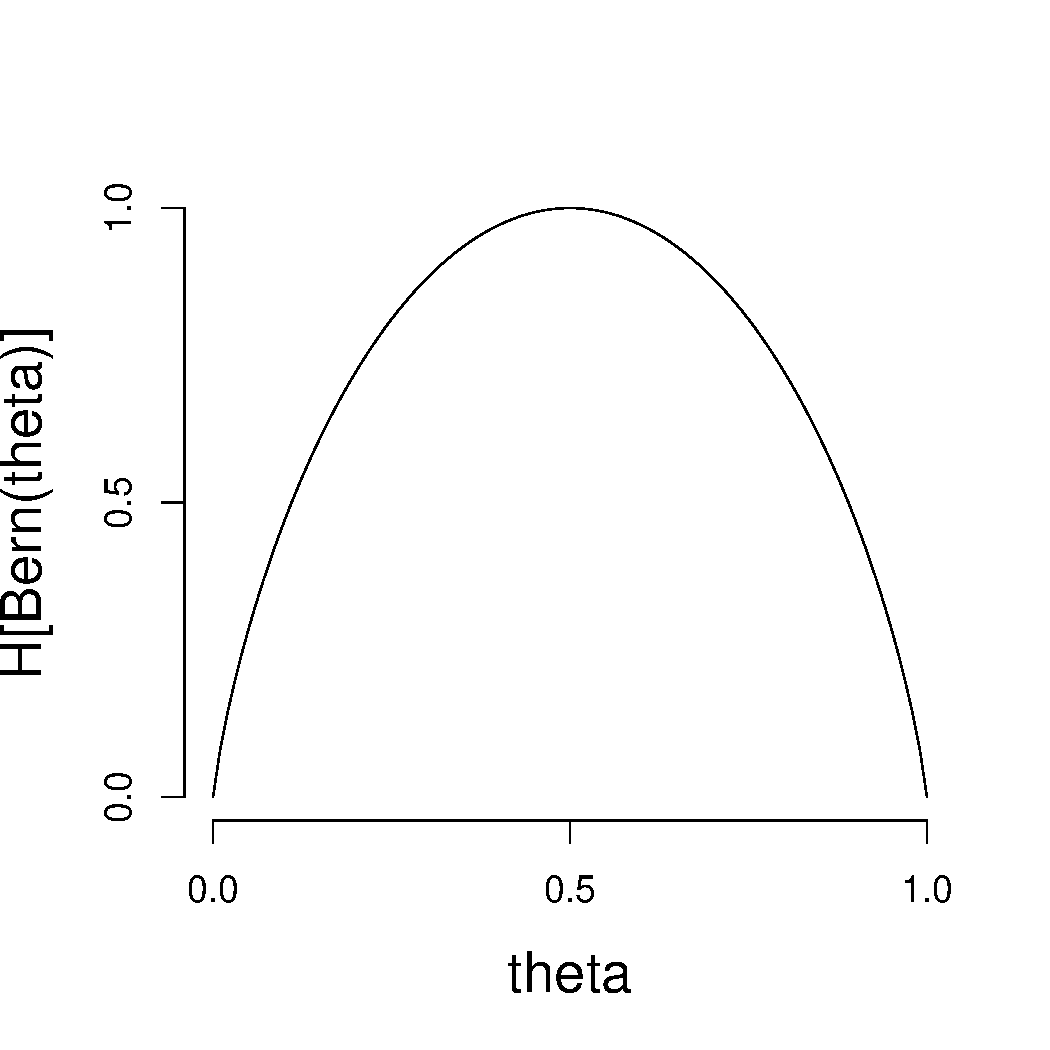
\includegraphics[height=1.75in]{pdfs/bern-entropy.pdf}
\end{center}%
\vspace*{-18pt}
\caption{Entropy of a random variable distributed as $\dbern{\theta}$.}\label{fig:bern-entropy}
\end{figure}
%
The graph makes it clear that when $\theta=0$ or $\theta=1$, the
outcome is certain, and therefore the entropy is 0.  The maximum
entropy possible for a Bernoulli distribution is 1 bit, achieved at
$\theta = 0.5$.  


\subsubsection{Entropy and Compression}

Entropy has a natural interpretation in terms of compression.  Suppose
we want to send the a message $X$ which might take on values in
$\nats$.%
%
\footnote{We can always code sequences of characters as numbers, as
originally noted by Kurt G\"odel, and as explained in any introductory
computer science theory text.  Just think of a string as representing
a number in the base of the number characters.}
%
If the sender and receiver both know the distribution $p_X$
of outcomes, the expected cost to send the message is $\entropy{X}$
bits.  For instance, if we need to send a bit with value 0 or 1, and
each outcome is equally likely, it will require 1 bit to send the
message.  On the other hand, if one outcome is more likely than the
other, we can save space (if we have repeated messages to send;
otherwise, we must round up).


\subsection{Joint Entropy}\label{section:stats-joint-entropy}

We can measure the entropy of two variables $X$ and $Y$ by measuring
the entropy of their joint distribution $p_{X,Y}$, generalizing our
definition to
%
\begin{equation}
\entropy{X,Y} = \expect{\log_2 p_{X,Y}(x,y)}.
\end{equation}
%
For instance, with discrete $X$ and $Y$, this works out to
%
\begin{equation}
\entropy{X,Y} = - \sum_{x} \sum_{y} p_{X,Y}(x,y) \ \log_2 p_{X,Y}(x,y).
\end{equation}
%

Joint entropy is symmetric, so that
%
\begin{equation}
\entropy{X,Y} = \entropy{Y,X}.
\end{equation}

\subsection{Conditional Entropy}\label{section:stats-conditional-entropy}

We can measure the entropy of a variable $X$ conditional on knowing
the value of another variable $Y$.  The expectation-based definition
is thus 
%
\begin{equation}
\condentropy{X}{Y} = \expect{-\log_2 p_{X|Y}(X|Y)}.
\end{equation}
%
In the case of discrete $X$ and $Y$, this works out to
%
\begin{align}
\condentropy{X}{Y} 
&= - \sum_y \sum_x p_{X,Y}(x,y) \ \log_2 p_{X|Y}(x|y)
\\
&= - \sum_y p_Y(y) \sum_x p_{X|Y}(x|y) \ \log_2 p_{X|Y}(x|y).
\end{align}
%

Conditional entropy, joint entropy and entropy are related as for
probabilty distributions, with
%
\begin{equation}
\entropy{X,Y} = \condentropy{X}{Y} + \entropy{Y}.
\end{equation}


\subsection{Mutual Information}\label{section:stats-mutual-information}

The mutual information between a pair of variables $X$ and $Y$ measures how
much more information there is in knowing their joint distribution than their
individual distributions for prediction.  Using expectations, mutual information
between variables $X$ and $Y$ is defined to be
%
\begin{align}
\mutualinfo{X}{Y} 
&= \expect{-\log_2 \frac{p_{X,Y}(x,y)}{p_X(x) \ p_Y(y)}}
&= \expect{-\log_2 p_{X,Y}(x,y)} + \expect{\log_2 p_X(x)} + \expect{\log_2 p_Y(y)}
\end{align}
%
In the discrete case, this unfolds to
%
\begin{equation}
\mutualinfo{X}{Y} = - \sum_{x,y} p_{X,Y}(x,y) \ \log_2 \frac{p_{X,Y}(x,y)}{p_X(x) \ p_Y(y)}.
\end{equation}
%

Mutual information is symmetric, so that
%
\begin{equation}
\mutualinfo{X}{Y} = \mutualinfo{Y}{X}.
\end{equation}
%
It's related to conditional and joint entropies by the unfolding
in the second step of the definition as 
%
\begin{align}
\mutualinfo{X}{Y} &= \entropy{X} + \entropy{Y} - \entropy{X,Y}
\\
&= \entropy{X} - \condentropy{X}{Y}.
\end{align}
%


\subsection{Divergence}\label{section:stats-divergence}

Kullback-Leibler (KL) divergence is the standard method to compare the
distributions of two random variables.  Pairs of topic distributions
that have similar probability assignments to words will have low KL
divergences from each other.

We will start with the discrete case, as it is what Griffiths and
Steyvers used in their experiments.  We'll consider the continuous
case, and specifically consider the Dirichlet distributions underlying
the LDA models.

\subsubsection{Cross Entropy}\label{section:stats-cross-entropy}

Cross entropy measures the ability of one distribution to represent
results drawn from another distribution.  Given two discrete random
variables $X$ and $Y$ with outcomes ranging from 1 to $N$, we define
the cross entropy of $X$ with respect to $Y$ as
%
\begin{equation}
\xentropy{X}{Y} = \sum_{n=1}^N p_X(n) \ \log_2 p_Y(n).
\end{equation}
%
This value measures the number of bits required, on average, to
transmit a value of $X$ using the distribution of $Y$ for coding.


\subsubsection{Defining KL Divergence}

As is standard, our definition will use random variables, but we point
out ahead of time that only the distributions of the variables matter,
not the outcomes.  Suppose that $X$ and $Y$ are two random variables
with possible outcomes ranging from 1 to $N$ and probabilty
distributions $p_X(n)$ and $p_Y(n)$.  The KL divergence of $X$ from
$Y$ is given by
%
\begin{equation}
\kld{X}{Y}
= \sum_{n=1}^N p_X(n) \log_2 \frac{p_X(n)}{p_Y(n)}.
\end{equation}
%
Because we used base-2 logs, the result is in units of bits.  Note
that this value is just the entropy of $X$ minus the cross entropy
of $X$ with respect to $Y$

If there is an outcome $n$ where $p_Y(n) = 0$ and $p_X(n) > 0$, the
divergence is infinite.  We may allow $p_X(n) = 0$ by interpreting $0
\log_2 \frac{0}{p_Y(n)} = 0$ by convention (even if $p_Y(n) > 0$).

Although we do not provide a proof, we note that $\kld{X}{Y} \geq 0$
for all random variables $X$ and $Y$.  We further note without proof
that $\kld{X}{Y} = 0$ if and only if $p_X = p_Y$.

For example, suppose we have three discrete random variables, $X$, $Y$
and $Z$, each with the same two outcomes, and distributions defined by
$p_X(1) = 0.2$, $p_X(2) = 0.8$ and $p_Y(1) = 0.4$, $p_Y(2) = 0.6$.  We
calculate 
%
\[
\kld{X}{Y} = 0.2 \log_2 (0.2/0.4) + 0.8 \log_2 (0.8/0.6) \approx 0.13.
\]
%
Consider a third random variable, $Z$, with $p_Z(1) = 0.5$ and
$p_Z(2) = 0.5$.  The KL-divergence calculation is 
%
\[
\kld{X}{Z} = 0.2 \log_2 (0.2/0.5) + 0.8 \log_2 (0.8/0.5) \approx 0.27.
\]
As we'd expect, $Z$ diverges further from $X$ than $Y$.  
Comparing $X$ to itself, we get
%
\[
\kld{X}{X} = 0.2 \log_2 (0.2/0.2) + 0.8 \log_2(0.8/0.8) = 0.
\]  
%
From this example, it's easy to see why $\kld{X}{X}$ is always 0.

KL divergence may expressed using expectation notation as
%
\begin{align}
\kld{X}{Y} 
&= \expect{\log_2 \frac{p_X(X)}{p_Y(X)}}
\\
&= \expect{\log_2 p_X(X)} - \expect{\log_2 p_Y(X)}.
\end{align}
%
As usual, unmarked expectation notation presupposes the natural
distributions for random variables, here using the distribution $p_X$
for the random variable $X$.%
%
\footnote{The first term is just the entropy of $X$,
$\entropy{X} = \expect{\log_2 p_X(X)}$.  Another way of interpreting
KL divergence is as the expected penalty in bits for using $p_Y$ to
model values of $X$ rather than $p_X$.}

\subsubsection{Symmetrized KL Divergence}\label{section:stats-symmetrized-kl-divergence}

KL divergence is not symmetric in the sense that there exist pairs of
random variables $X$ and $Y$ such that $\kld{X}{Y} \neq \kld{Y}{X}$.
We have an example to hand.  Consider our example $X$ and $Y$ above,
for which we noted $\kld{X}{Y} \approx 0.13$.  The other way around,
$\kld{Y}{X} = 0.4 \log_2 0.4/0.2 + 0.6 \log_2 0.6/0.8 \approx 0.15$.

There are several divergence measures derived from KL divergence that
are symmetric.  The simplest approach is just to introduce symmetry
by brute force.  The symmetrized KL-divergence between random variables
$X$ and $Y$ is defined by averaging KL divergence of $X$ from $Y$
and of $Y$ from $X$,
%
\begin{equation}
\skld{X}{Y} = \frac{1}{2}(\kld{X}{Y} + \kld{Y}{X}).
\end{equation}
%
Obviously, $\skld{X}{Y} = \skld{Y}{X}$, so the measure is symmetric.


\subsubsection{Jensen-Shannon Divergence}

Another widely used symmetric divergence measure derived from KL divergence
is the Jensen-Shannon divergence.  To compare $X$ and $Y$ using Jensen-Shannon
divergence, we first define a new random variable $Z$ with distribution defined by
averaging the distributions of $X$ and $Y$,
%
\[
p_Z(n) = \frac{1}{2}(p_X(n) + p_Y(n)).
\]
%
We then define Jensen-Shannon divergence by taking average divergence
from $Z$,
%
\begin{equation}
\jsd{X}{Y} = \frac{1}{2}(\kld{X}{Z} + \kld{Y}{Z}).
\end{equation}
%
As with the symmetrized KL divergence, Jensen-Shannon divergence is
symmetric by definition.


\subsubsection{LingPipe KL-Divergence Utilities}

KL-divergence is implemented as a static utility method in the
\code{Statistics} utility class in package \code{com.aliasi.stats}.
The method takes two double arrays representing probability
distributions and measures how much the first is like the second.

In order to give you a sense of KL-divergence, we implement a simple
utility in the demo class \code{KlDivergence} to let you try various
values.  The code just parses out double arrays from teh command line
and sends them to the KL function.
%
\codeblock{KlDivergence.1}

The ant target \code{kl} runs the command with the first two arguments
given by properties \code{p.x} and \code{p.y}.  To calculate the example
from above, we have
%
\commandlinefollow{ant -Dp.x="0.2 0.8" -Dp.y="0.4 0.6" kl}
\begin{verbatim}
pX=(0.2, 0.8)     pY=(0.4, 0.6)     
kld=0.13202999942307514    
skld=0.1415037499278844   
jsd=0.03485155455967723
\end{verbatim}
%
The Jensen-Shannon divergence is less than the symmetrized KL
divergence because the interpolated distribution $p_Z$ is closer to
both of the original distributions $p_X$ and $p_Y$ than they are to
each other.

